% Agent–Environment interaction diagram – PPT colour scheme (v5)
% Schematic but friendly and approachable
% Compile: xelatex agent_environment_tikz_v5.tex
% Convert: pdf2svg agent_environment_tikz_v5.pdf agent_environment_tikz_v5.svg
\documentclass[border=10pt]{standalone}
\usepackage{fontspec}
\setmainfont{Aptos}[
  Path = /Applications/Microsoft Word.app/Contents/Resources/DFonts/,
  Extension = .ttf,
  UprightFont = Aptos,
  BoldFont = Aptos-Bold,
  ItalicFont = Aptos-Italic,
  BoldItalicFont = Aptos-Bold-Italic,
]
\usepackage{amsmath,amssymb}
\usepackage{tikz}
\usetikzlibrary{arrows.meta, calc}

% PPT colours
\definecolor{accent}{HTML}{CB8044}
\definecolor{fg}{HTML}{E8E8E8}
\definecolor{fgdim}{HTML}{AAAAAA}
\definecolor{accentfaint}{HTML}{CB8044}
% Globe colours
\definecolor{land}{HTML}{7BA656}
\definecolor{ocean}{HTML}{5C85A8}

\begin{document}
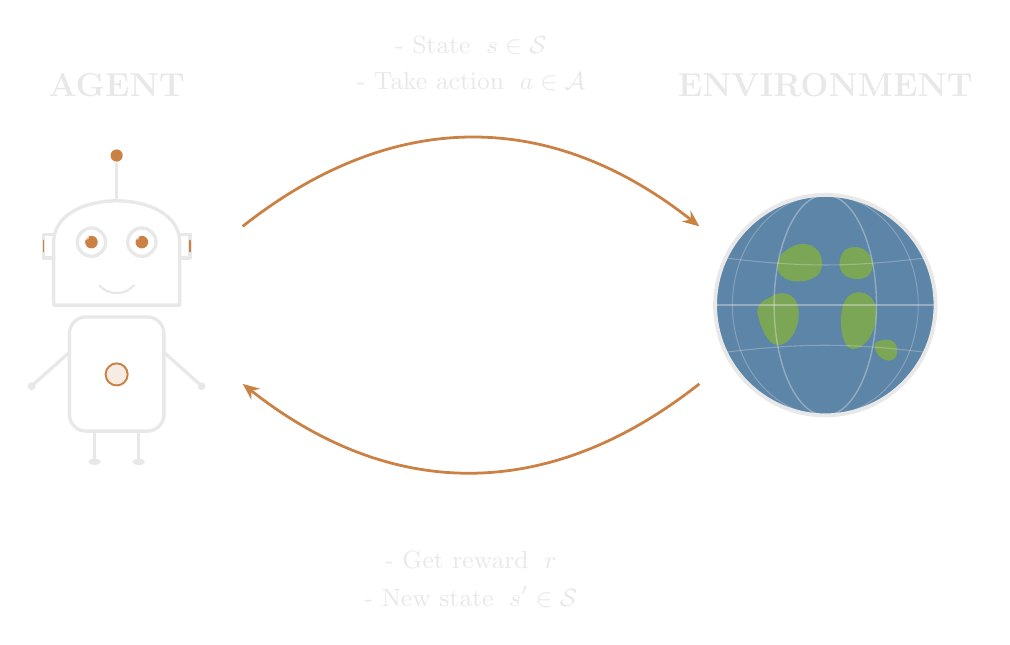
\begin{tikzpicture}[
    >=Stealth,
    curvedarrow/.style={
        accent,
        line width=1pt,
        -{Stealth[length=6pt, width=5pt]},
    },
]

% =============================================
% AGENT – Schematic robot, friendly
% Same wireframe style as v1, but with:
%   - rounded head (dome top instead of sharp rectangle)
%   - gentle smile instead of grid mouth
%   - slightly larger eyes with warm pupils
%   - round hand/feet caps
% =============================================
\begin{scope}[shift={(0,0)}, fg, line width=1.2pt, line cap=round, line join=round]

  % Head – narrower, dome top
  \draw (-0.8,0.5) -- (-0.8,1.3)
    .. controls (-0.8,2.0) and (0.8,2.0) .. (0.8,1.3)
    -- (0.8,0.5) -- (-0.8,0.5);

  % Antenna stem
  \draw (0,1.85) -- (0,2.3);
  % Antenna tip
  \fill[accent] (0,2.4) circle (2.2pt);

  % Eyes – friendly, proportionate
  \draw (-.32,1.3) circle (0.18);
  \fill[accent] (-.32,1.3) circle (0.08);
  \fill[white, opacity=0.6] (-0.38,1.36) circle (0.03);
  \draw (.32,1.3) circle (0.18);
  \fill[accent] (.32,1.3) circle (0.08);
  \fill[white, opacity=0.6] (0.26,1.36) circle (0.03);

  % Smile
  \draw[line width=0.8pt] (-0.22,0.75) .. controls (-0.1,0.62) and (0.1,0.62) .. (0.22,0.75);

  % Body – slimmer, taller
  \draw[rounded corners=6pt] (-0.6,-1.1) rectangle (0.6,0.35);

  % Body accent – warm circle
  \draw[accent, line width=0.7pt] (0,-0.38) circle (0.14);
  \fill[accent, opacity=0.15] (0,-0.38) circle (0.14);

  % Arms – angled lines with round hand caps
  \draw (-0.6,-0.1) -- (-1.05,-0.5);
  \fill[fg] (-1.08,-0.53) circle (0.05);
  \draw (0.6,-0.1) -- (1.05,-0.5);
  \fill[fg] (1.08,-0.53) circle (0.05);

  % Legs – with round feet
  \draw (-0.28,-1.1) -- (-0.28,-1.45);
  \fill[fg] (-0.28,-1.49) ellipse (0.08 and 0.04);
  \draw (0.28,-1.1) -- (0.28,-1.45);
  \fill[fg] (0.28,-1.49) ellipse (0.08 and 0.04);

  % Ears – small side details
  \draw (-0.8,1.1) -- (-0.93,1.1) -- (-0.93,1.4) -- (-0.8,1.4);
  \draw[accent, line width=0.6pt] (-0.93,1.18) -- (-0.93,1.32);
  \draw (0.8,1.1) -- (0.93,1.1) -- (0.93,1.4) -- (0.8,1.4);
  \draw[accent, line width=0.6pt] (0.93,1.18) -- (0.93,1.32);

\end{scope}

% Agent label
\node[fg, font=\fontsize{12}{14}\selectfont\bfseries] at (0,3.3) {AGENT};

% =============================================
% ENVIRONMENT – Schematic globe with colours (from v3/v4)
% =============================================
\begin{scope}[shift={(9,0.5)}]
  % Ocean fill
  \fill[ocean] (0,0) circle (1.4);

  % Land mass blobs
  \fill[land] (-0.55,0.65)
    .. controls (-0.35,0.85) and (-0.1,0.8) .. (-0.05,0.6)
    .. controls (0.0,0.4) and (-0.15,0.3) .. (-0.35,0.3)
    .. controls (-0.55,0.3) and (-0.7,0.45) .. (-0.55,0.65);
  \fill[land] (0.25,0.7)
    .. controls (0.4,0.8) and (0.6,0.7) .. (0.6,0.5)
    .. controls (0.6,0.35) and (0.45,0.3) .. (0.3,0.35)
    .. controls (0.15,0.4) and (0.15,0.6) .. (0.25,0.7);
  \fill[land] (0.35,0.15)
    .. controls (0.5,0.2) and (0.65,0.1) .. (0.65,-0.1)
    .. controls (0.65,-0.3) and (0.55,-0.5) .. (0.4,-0.55)
    .. controls (0.25,-0.6) and (0.2,-0.4) .. (0.2,-0.2)
    .. controls (0.2,0.0) and (0.25,0.1) .. (0.35,0.15);
  \fill[land] (-0.7,0.1)
    .. controls (-0.55,0.2) and (-0.4,0.15) .. (-0.35,0.0)
    .. controls (-0.3,-0.2) and (-0.4,-0.45) .. (-0.55,-0.5)
    .. controls (-0.7,-0.55) and (-0.8,-0.35) .. (-0.85,-0.15)
    .. controls (-0.9,0.0) and (-0.8,0.05) .. (-0.7,0.1);
  \fill[land] (0.7,-0.45)
    .. controls (0.85,-0.4) and (0.95,-0.5) .. (0.9,-0.65)
    .. controls (0.85,-0.75) and (0.7,-0.7) .. (0.65,-0.6)
    .. controls (0.6,-0.5) and (0.62,-0.47) .. (0.7,-0.45);

  % Schematic grid lines
  \draw[fg, line width=0.5pt, opacity=0.4] (0,-1.4) arc[start angle=-90, end angle=90, x radius=0.65, y radius=1.4];
  \draw[fg, line width=0.5pt, opacity=0.4] (0,1.4) arc[start angle=90, end angle=270, x radius=0.65, y radius=1.4];
  \draw[fg, line width=0.35pt, opacity=0.3] (0,-1.4) arc[start angle=-90, end angle=90, x radius=1.18, y radius=1.4];
  \draw[fg, line width=0.35pt, opacity=0.3] (0,1.4) arc[start angle=90, end angle=270, x radius=1.18, y radius=1.4];
  \draw[fg, line width=0.5pt, opacity=0.4] (-1.4,0) -- (1.4,0);
  \draw[fg, line width=0.4pt, opacity=0.3] (-1.28,0.6) .. controls (-0.3,0.48) and (0.3,0.48) .. (1.28,0.6);
  \draw[fg, line width=0.4pt, opacity=0.3] (-1.28,-0.6) .. controls (-0.3,-0.48) and (0.3,-0.48) .. (1.28,-0.6);

  % Globe outline
  \draw[fg, line width=1.4pt] (0,0) circle (1.4);
\end{scope}

% Environment label
\node[fg, font=\fontsize{12}{14}\selectfont\bfseries] at (9,3.3) {ENVIRONMENT};

% =============================================
% TOP ARROW: Agent -> Environment
% =============================================
\draw[curvedarrow]
    (1.6,1.5) .. controls (3.5,3.0) and (5.5,3.0) .. (7.4,1.5);

% Top labels – placed above the arrow arc
\node[fg, font=\fontsize{9}{11}\selectfont, anchor=south] at (4.5,3.55) {%
  - State\; $s \in \mathcal{S}$%
};
\node[fg, font=\fontsize{9}{11}\selectfont, anchor=south] at (4.5,3.1) {%
  - Take action\; $a \in \mathcal{A}$%
};

% =============================================
% BOTTOM ARROW: Environment -> Agent
% =============================================
\draw[curvedarrow]
    (7.4,-0.5) .. controls (5.5,-2.0) and (3.5,-2.0) .. (1.6,-0.5);

% Bottom labels – placed below the arrow arc
\node[fg, font=\fontsize{9}{11}\selectfont, anchor=north] at (4.5,-2.5) {%
  - Get reward\; $r$%
};
\node[fg, font=\fontsize{9}{11}\selectfont, anchor=north] at (4.5,-2.95) {%
  - New state\; $s' \in \mathcal{S}$%
};

\end{tikzpicture}
\end{document}
